\subsection{Logarithmic Photoreceptor}

There exists several types of logarithmic photoreceptor circuits that exhibit different properties, these are shown in figure \ref{fig:Log_Photoreceptors}. 

\begin{figure}[H]
    \centering
    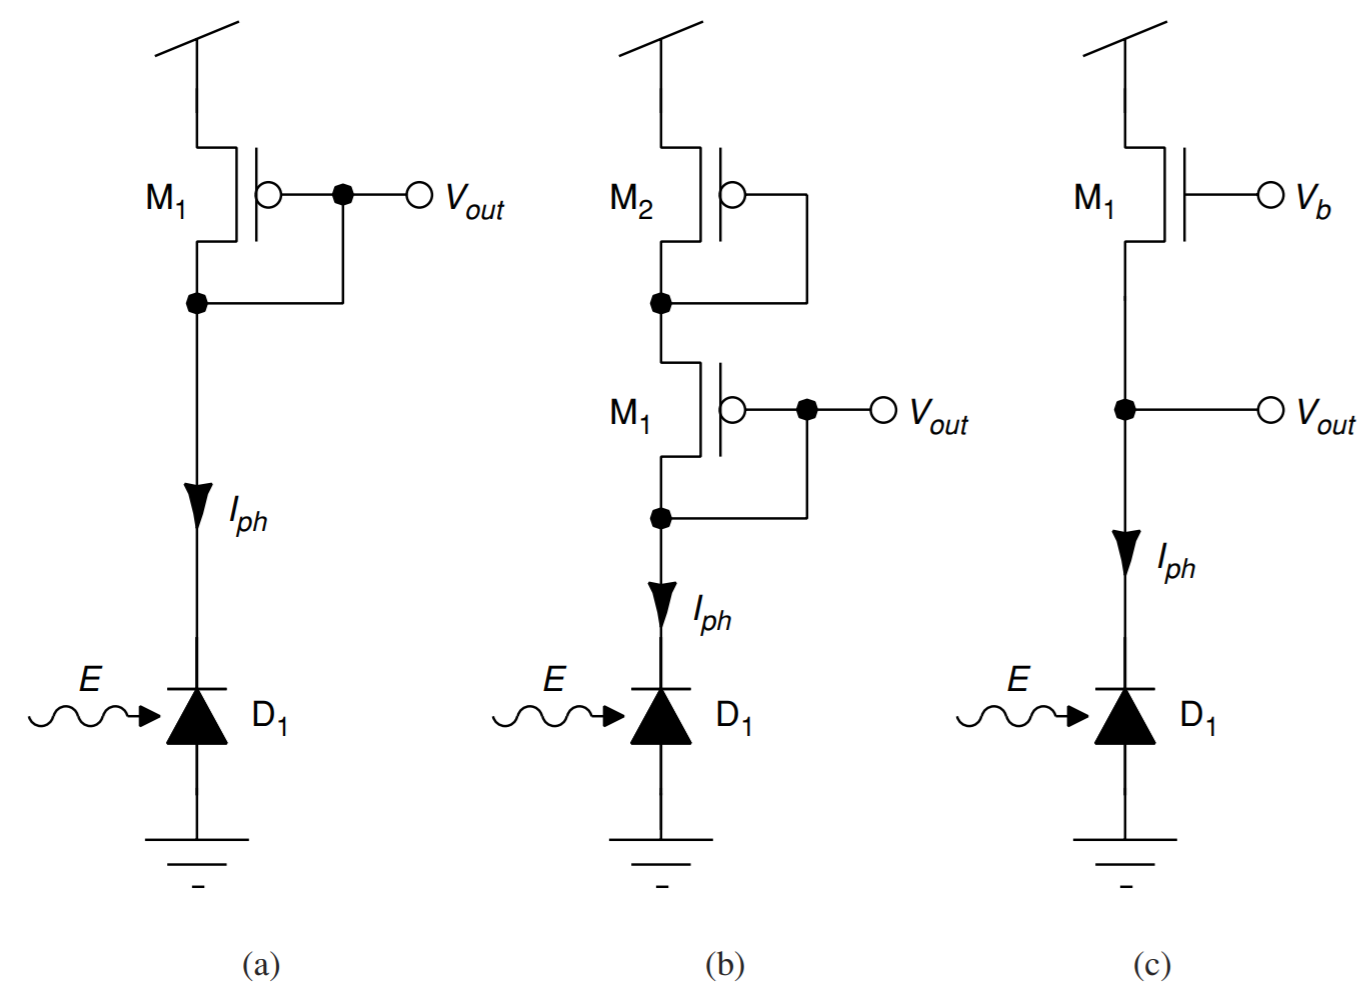
\includegraphics[width=0.5\linewidth]{../../Figures/Log_Photoreceptors.PNG}
    \caption{Photosensors with logarithmic irradiance-to-voltage conversion for subthreshold photocurrents, consisting of a photodiode and a current-to-voltage conversion stage implemented as (a) a diodeconnected MOSFET, (b) two diode-connected MOSFETs in series, (c) a MOSFET in sourcefollower configuration. Adapted from Textbook.}
    \label{fig:Log_Photoreceptors}
\end{figure}

I include the transfer functions for these circuits here without derivation. This is typically the kind of things that I believe they may ask us to derive in the exam, though I leave it as an exercise for the reader :). 

\begin{equation}
    \mathrm{Diode \ Connected:}\ V_{out} = V_{dd} - \frac{U_T}{\kappa}\mathrm{log}(\frac{I_{ph}}{I_0})
\end{equation}
\begin{equation}
    \mathrm{Double \ Diode \ Connected:}\ V_{out} = V_{dd} - U_T\frac{\kappa + 1}{\kappa ^2}\mathrm{log}(\frac{I_{ph}}{I_0})
\end{equation}
\begin{equation}
    \mathrm{Source \ Follower:}\ V_{out} = \kappa V_g - U_T\mathrm{log}(\frac{I_{ph}}{I_0})
\end{equation}

UNCLEAR: $I_{ph}$ is the "static scene illuminance" (in Lux).   

\subsection{Reasoning through Source Follower Logarithmic Photoreceptor}

Now let's look in details at the circuit that we have studied in class and that we most likely will be asked about: the source follower photoreceptor 

\begin{figure}[H]
    \centering
    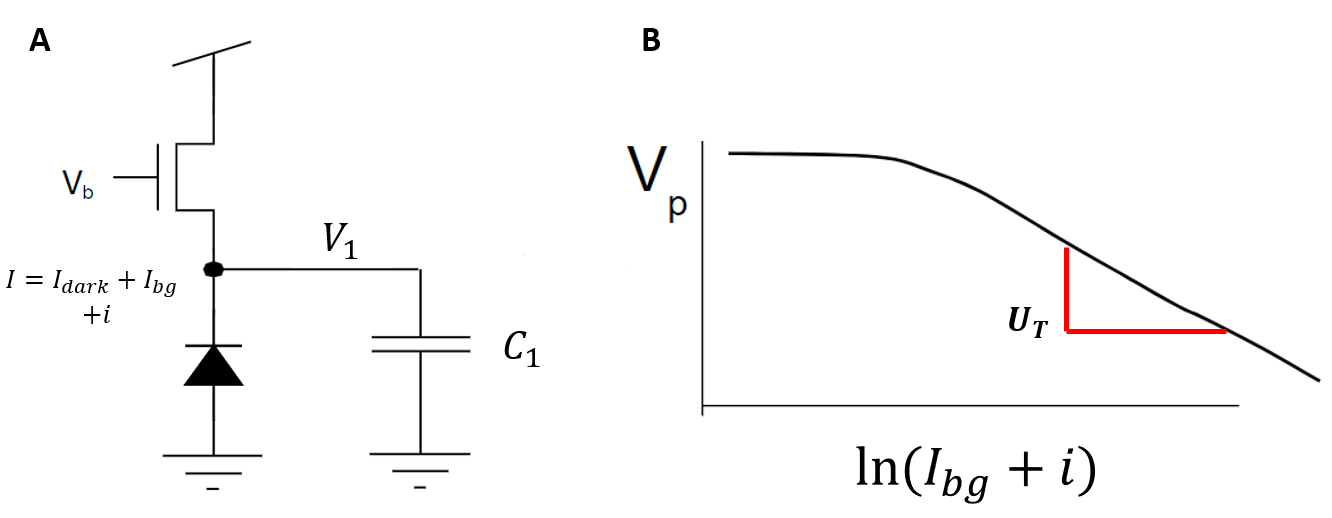
\includegraphics[width=0.8\linewidth]{../../Figures/Souce_Follower_Photoreceptor.PNG}
    \caption{Source Follower Circuit with parasitic capacitance considered. $I_{dark}$ is the constant dark current, $I_{bg}$ the static scene luminance $i$ signal luminance (varying part). Resulting current I = $I_{dark} + I_{bg} + i = I_0e^{\frac{\kappa V_b - V_1}{U_T}}$. Adapted from Lecture notes.}
    \label{fig:Souce_Follower_Photoreceptor}
\end{figure}

The difference between the circuit shown in figure \ref{fig:Souce_Follower_Photoreceptor} and  figure \ref{fig:Log_Photoreceptors}.C is the capacitor. In reality, the capacitance is also present in figure \ref{fig:Souce_Follower_Photoreceptor}.C (A and B as well for the matter) but it is omitted from the schematic. The capacitance that you see is the "parasitic capacitance" which we have already encoutered before. It is indeed present in all electrical components and need sometimes be considered. This is the case here as we need to consider the speed at which response is obtained, which is an obviously important criteria for photosensors. 

Let's first analyze the source follower circuit. Tobi's explanation on the topic is extremely clear, so I'll just copy (almost) word to word what he said in the lecture. It's best to proceed step by step, so let's do it like this: 

\begin{enumerate}
    \item When light shines on the photodiode you see, a current is generated. This current is linearly proportional to the incident light.
    \item If there is no light, you have some dark current. 
    \item When light shines, because of conventional current source, the photodiode acts as a constant current \textit{sink}.
    \item When light shines, the photodiode sinks currents, and in way, \textit{forces} the current to sink. That means that the top transistor is forced to adapt itself to match the current from the photodiode. As we assume that the gate voltage is unchanged, the source voltage of our top transistor ($V_1$/$V_p$) must change to match the photodiode. The more light shines, the higher the current, and hence the lower $V_1$/$V_p$ need to be (to reach a higher $V_{gs}$. We can thus write the following equations, by taking $I$ as the current flowing through the photodiode, equal to the dark current + the photocurrent:
    \begin{equation}
        I_0e^{\frac{\kappa V_b - V_1}{U_T}} = I
    \end{equation}
    \item Since the current flowing in  in the transistor is \textit{exponential} to the $V_{gs}$, then it follows the the source voltage changes in \textit{logarithmic} fashion with the changing current.This yields@
    \begin{equation}
        V_1 = \kappa V_b - U_T\mathrm{ln}(\frac{I}{I_0})
    \end{equation}
    We can also derive from this the graph which is seen in \ref{fig:Souce_Follower_Photoreceptor}, the slope of the linear part is $U_T$
    \item Every photodiode has an associated parasitic capacitance associated to it - this also happens to low pass filter the signal here (because there is a conductance at the node and then the capacitace, so it's an RC configuration). 
    \item There is thus a time constant associated with the node, which is related to the capacitance and the conductance of the node. The conductance of the node is "how much does the current in the node change when changing the voltage".
    \item To evaluate the conductance, let's remember that the photodiode behaves like a constant current sink (assuming constant light), so this current does not change with the voltage ($V_p$). However, the current in the transistor is heavily (exponentially) controlled by the voltage ($V_p$). 
    \item The source conductance is therefore simply the "source conductance" of the subthreshold transistor, which we've derived before. This is $g_s = I/U_T$.
    \item We thus now have the time constant of our circuit: $\tau = RC = C/G = \frac{C\cdot U_T}{I}$. 
    \item The time constant is inversely proportional to the photocurrent. In other words, \textbf{the brighter the light, the faster the circuit behaves}. This is a problem because it means our circuit will not behave properly in low light conditions. To deal with this problem, we typically go for a more practical transimpedance log photoreceptor. 
\end{enumerate}

\subsubsection{Time domain response of source follower response}

\begin{enumerate}
    \item The current flowing through the capacitor must be the current sinked by the photodiode minus the current flowing through the transistor. Let's omit $U_T$ for simplicity. 
    \begin{equation}
        C \dot{v_1}\footnote{Dot means derivative - here with respect to time} = e^{\frac{\kappa V_b - V_1}{U_T}} - I
    \end{equation}
    \item Small signal analysis yields:
    \begin{equation}
        C \dot{v_1} = -g_sv_1-i
    \end{equation}
    \item Knowing that $\tau = c/g_s$, we have the transfer function:
    \begin{equation}
        (\tau s + 1)v_1 = -\frac{i}{g_s}
    \end{equation}
    If we compute the magnitude of the transfer function:
    \begin{equation}
        |\frac{v1}{i/g_s}| = |\frac{1}{\tau s + 1}|
    \end{equation}
    This is the transfer function of a \textbf{lowpass filter!} Note that the input is current and we obtain volts, which is why we speak of transconductance $g_s$.
    
\end{enumerate}


